\documentclass[12pt]{article}
\usepackage{graphicx}         % fuer das Einbinden von Grafiken
\usepackage{float}    % für Grafiken, um [H] zu verwenden
\usepackage[ngerman]{babel}   % weglassen, wenn in Englisch
%% wenn Sie das ngerman package benutzen, koennen Umlaute als "a.. geschrieben
%% werden, sonst \"a..
\usepackage[utf8x]{inputenc}
%% dieses package erlaubt, bei deutscher Tastatur Umlaute, ß direkt einzugeben
\usepackage[LGRgreek]{mathastext}
%% kursiv in Formeln nicht verwenden

\textwidth=170mm
\textheight=250mm
\hoffset= -20mm       % may need change
\voffset= -30mm       % may need change

%% everything after % is a comment in LATEX

\begin{document}

%% we do the title page ourselves
\thispagestyle{empty}     % only for frontpage
\null\vspace{40mm}
\begin{center}
{%%%%%%%%%%%%%%%%%%%%%%%%%% Titel
\Large  Gasaustausch - Wechselwirkung zwischen Ozean und Atmosph\"are
\footnote{\noindent Versuch F54, ausgef\"uhrt am 10.08.2017, Betreuer Kerstin Krall, lange besondere Auswertung}
}\\[15mm]
%%%%%%%%%%%%%%%%%%%%%%%%%%% Authors
C. Blattgerste und J. Ziegler

\vspace{25mm}

\parbox{0.9\textwidth}{   %% etwas schmaler als normaler Satz

\small The aim of the experiment is to get an insight into $CO_2$ gas exchange between the atmosphere and the ocean. For this purpose, the exchange rate of carbon dioxide between air and water is measured by use of conductivity and pH measurements in an annular wind-wave channel. The pH value is determined by use of pH indicators and optical absorption spectroscopy. By measuring different parameters at different times it is possible to compare them to the given theory.
}
\end{center}

\vfill
Als besondere Auswertung testiert: Datum, Unterschrift:
\vspace{20mm}

%% Rueckseite des Titelblatts leer. Bei einseitigem Druck entfernen
\newpage
\null\thispagestyle{empty}

\newpage     % Inhaltsverzeichnis, koennte man bei langer Version machen
\tableofcontents
\addtocontents{toc}{\vspace{\baselineskip}}
\newpage

\section{Einleitung}

Da die Erdoberfläche zu knapp 70\% aus Wasser besteht, ist es für den globalen Gasaustausch und das Gesamtklima essentiell, die zugrunde liegenden Prinzipien eines Gasaustauschs zwischen Ozean und Atmosphäre zu untersuchen und zu verstehen.

Um die Mechanismen genau verstehen zu können, eignen sich Feldversuche nur bedingt, da dort die Parameter der Experimente nicht gezielt beeinflusst werden können. Das Experiment wird deshalb speziell in einem Wind-Wellen-Kanal durchgeführt. Einführend soll deshalb etwas Grundlagenwissen für den Versuch diskutiert werden.

Wichtig zu wissen ist, dass die Transfergeschwindigkeit für den Gasaustausch zu großen Teilen von Wind, Wellen und Oberflächenfilmen abhängt. Dies wird teilweise im Folgenden untersucht. In der Grenzschicht zwischen den beiden aufeinandertreffenden Fluiden ist für den Transport des Gases hauptsächlich Diffusion verantwortlich, fernab davon vorwiegend Turbulenzen. Die Grenzschicht beschreibt dabei den Übergang zwischen zwei Medien unterchiedlicher Dichte, wobei deren Dicke hier als etwa $1 mm$ angenommen werden kann.
Da auch der Einfluss der Zusammensetzung des Wassers verstanden werden soll, werden bei dem Experiment außerdem zwei verschiedene Flüssigkeiten vermessen: vollentsalzenes Wasser (VE-Wasser) und mit $NaOH$ versetztes VE-Wasser, was hier Meerwasser modelliert, da dieses auf natürliche Weise leicht basisch ist. Um Konzentrationsänderungen von $CO_2$ schließlich bestimmen zu können, sind geeignete Messverfahren notwendig. Hier angewendet wird die Leitfähigkeitsmethode und die Indikator-Methode, welche an gegebener Stelle im Detail aufgegriffen werden.

In diesem Versuch sollen die Messdaten vorrangig mit dem einfachen Boxmodell ausgewertet und verglichen werden. Dort werden die zwei Fluide als jeweils ein Rechteck dargestellt und dadurch ist es möglich das ganze System durch eine einfach Exponentialgleichung zu beschreiben. Die detailierte Erklärung des Modells folgt im Theorieteil.

\section{Theorie}

\subsection*{k-Wert}
\subsection{Messmethoden}
\subsection{title}

\subsection{Boxmodell}
Erwähnt werden soll jedoch noch das Boxmodell, welches für die Berechnungen von entscheidender Bedeutung ist. Hierbei wird der Luft- und Wasserraum als jeweils eine separate Box betrachtet. Diese sind durch Parameter, wie die Konzentration des Gases beschrieben. Unter geeigneten Annahmen, welche teilweise in den Ergebnissen genauer betrachtet werden, ergibt sich bei einer Evasion, also dem Übergang von $CO_2$ aus dem Wasser in die Luft, ein Verhalten der Konzentration von $CO_2$ im Wasser, welches sich durch folgende Formel zeitlich beschreiben lässt:

\begin{equation}
c_w(t) = c_w(0) \, exp\Big(- \frac{k}{h_{eff}}t\Big)
\end{equation}
Auch auf diese wird in den Ergebnissen noch genauer eingegangen.








\section{Versuchsanordnung}

\begin{figure}[H]
	\centering
	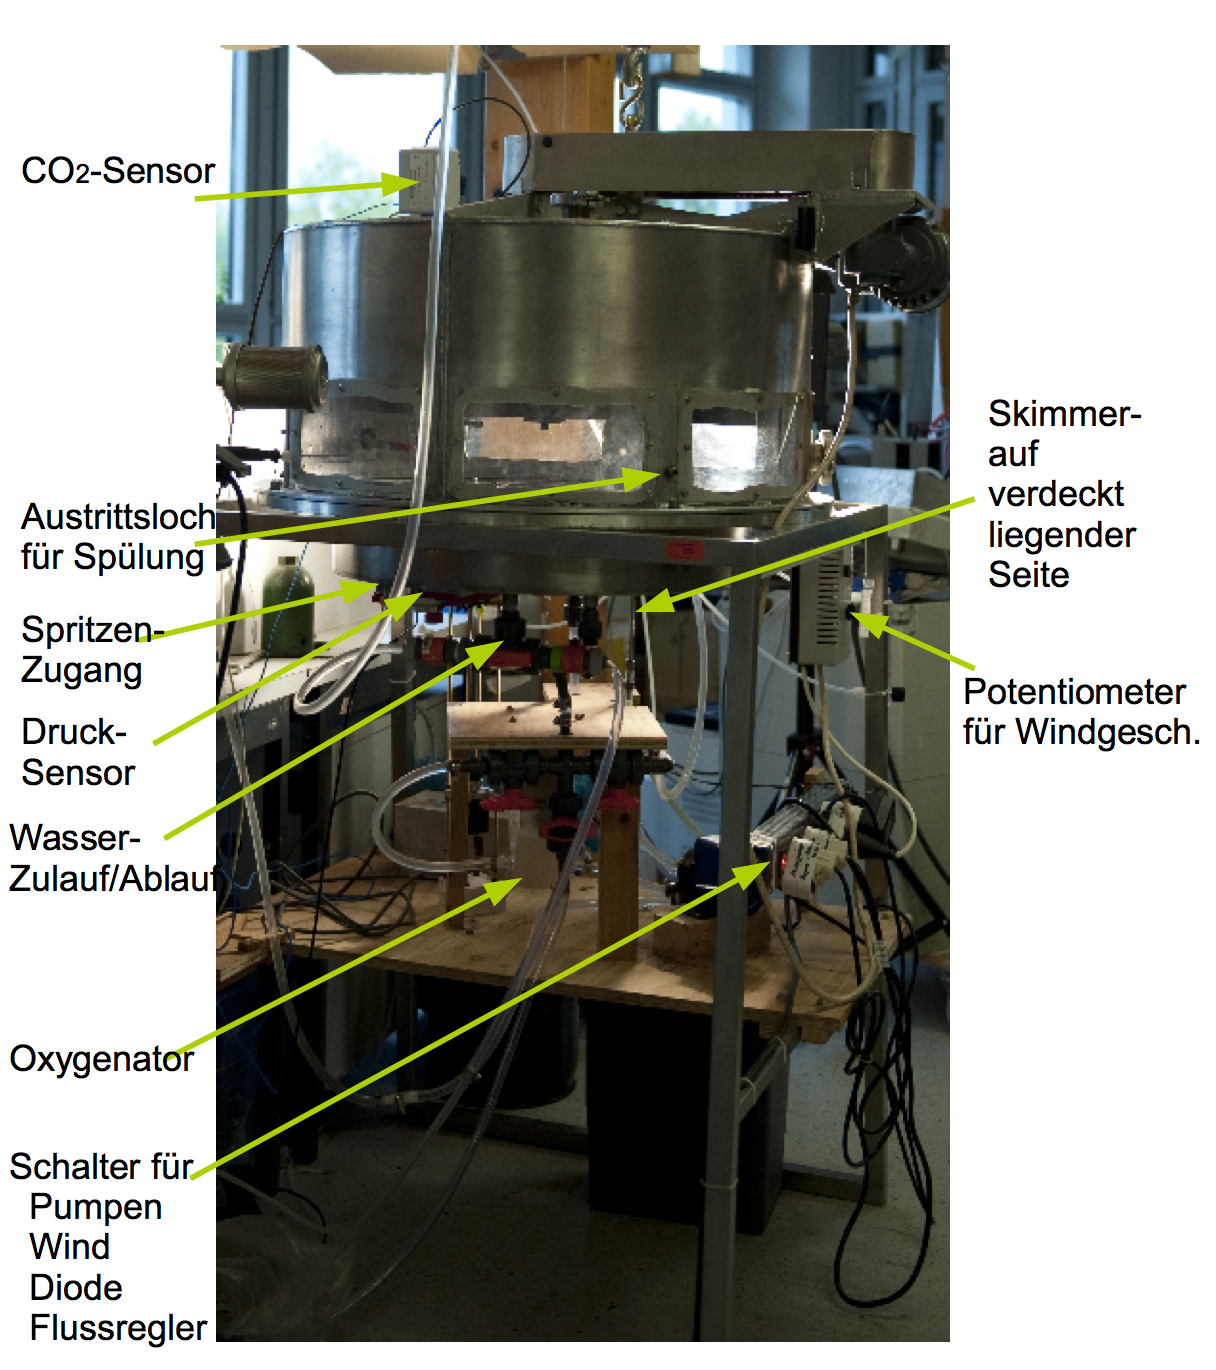
\includegraphics[width=70mm]{Versuchsaufbau}
	\caption{Übersicht über den Versuchsaufbau (Abbildung 10 \cite{jaehne})}
\end{figure}

Wie in der Übersicht zu sehen ist, wird der Versuch in einem ringförmigen Wind-Wellen-Kanal durchgeführt. Für beide Versuchsteile wird vollentsalztes Wasser verwendet. Hierbei handelt es sich um normales Haushaltswasser, was zusätzlich noch mit einem Ionentauscher aufbereitet wurde. Die Füllhöhe der Wasserrinne wird während des Versuchs mit einem Drucksensor über den hydrostatischen Druck gemessen. Der Luftraum wird ständig mit $CO_2$-freier Luft aus einem Reinstluftgenerator gespült. Dies führt zu einem leichten Unterdruck im Kanal, was in der Folge dazu führt, dass keine verunreinigte Umgebungsluft einströmen kann. Temperatur und $CO_2$-Konzentration werden mit handelsüblichen Sonden aufgenommen und vom PC ausgelesen. Für die Erzeugung des Windes stehen vier motorbetriebene Rotorblätter zur Verfügung. Diese kreisen im Luftraum. Über die Motorleistung kann die Windgeschwindigkeit reguliert werden. Der auch im Versuchsaufbau eingezeichnete Oxygenator dient dazu das Wasser mit Gas, in diesem Fall $CO_2$, anzureichern. Seine Funktionsweise ähnelt der einer Lunge. Anschließend wichtig zu nennen ist noch der Skimmer, welcher verwendet wird, um einen evtl. auftretenden Oberflächenfilm vom Wasser absaugen zu können.

\section{Versuchsdurchf\"uhrung}

Zunächst ist anzumerken, dass der Versuch grundsätzlich zwei mal durchgeführt wurde. Das jeweils verwendete Wasser war einmal VE-Wasser und im zweiten Teil Meermodellwasser. Zur Symolation des Meerwassers werden $2.5ml$ einer 1-molaren $NaOH$-Lösung in das gesammte im Wasserkanal befindliche Wasservolumen gegeben.
Nachfolgend soll nur auf die wichtigsten Schritte während des Experiments eingegangen werden. Im Versuchsheft wurde handschriftlich Protokoll über die einzelnen Teile geführt:
1. Prüfen der Leitfähigkeit des verwendeten Wassers, um sicherstellen zu können, dass unter einem bestimmten Schwellenwert. 2. Aufnahme von Lampenspektren 3. Für den Versuchsteil mit Meermodellwasser wird Natriumhydroxid dem Wasser hinzugegeben. 4. Begasung des Wassers mit $CO_2$ 5. Evasionsmessung 6. Alkalisches und saures Referenzspektrum aufnehmen, sowie Dunkelspektrum.

\section{Auswertung/Ergebnisse}
\subsection{VE-Wasser}
\subsubsection{Zeitliche Verl\"aufe der Messdaten}

\begin{figure}[H]
	\centering
	% hier schon der komplixiert Fall, dass 2 Bilder nebeneinander gesetzt werden
	\parbox{82.5mm}{
		\centering
		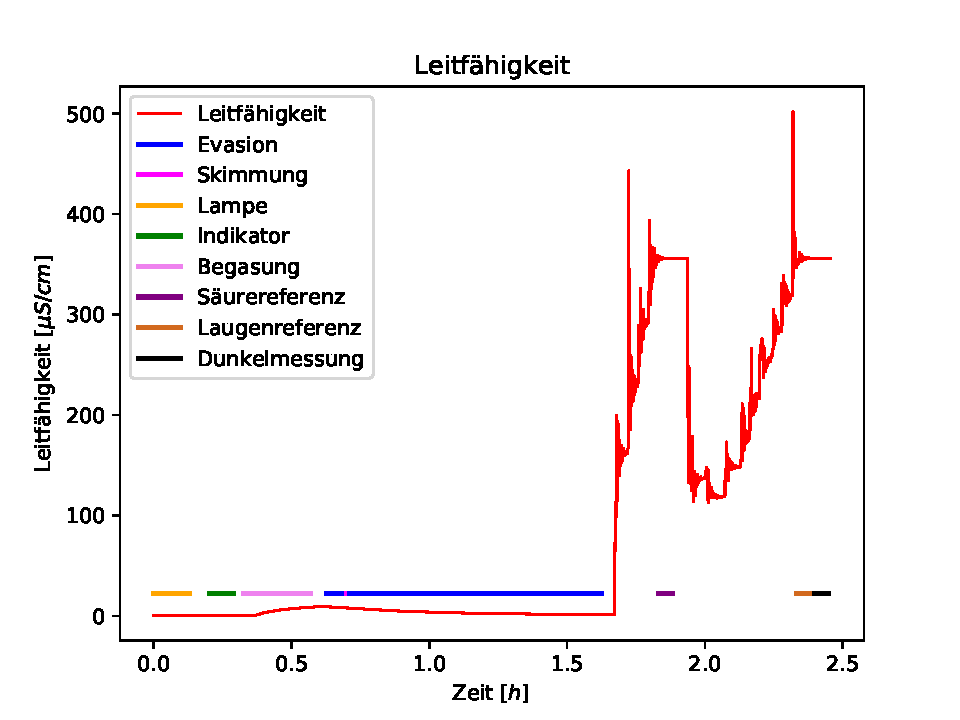
\includegraphics[width=82.5mm]{VE-Wasser/Leitfaehigkeit}
		\caption{Leitf\"ahigkeit}
	}
	\hfill% fuegt Platz ein, das rueckt die beiden Bilder an den Rand
	\parbox{82.5mm}{
		\centering
		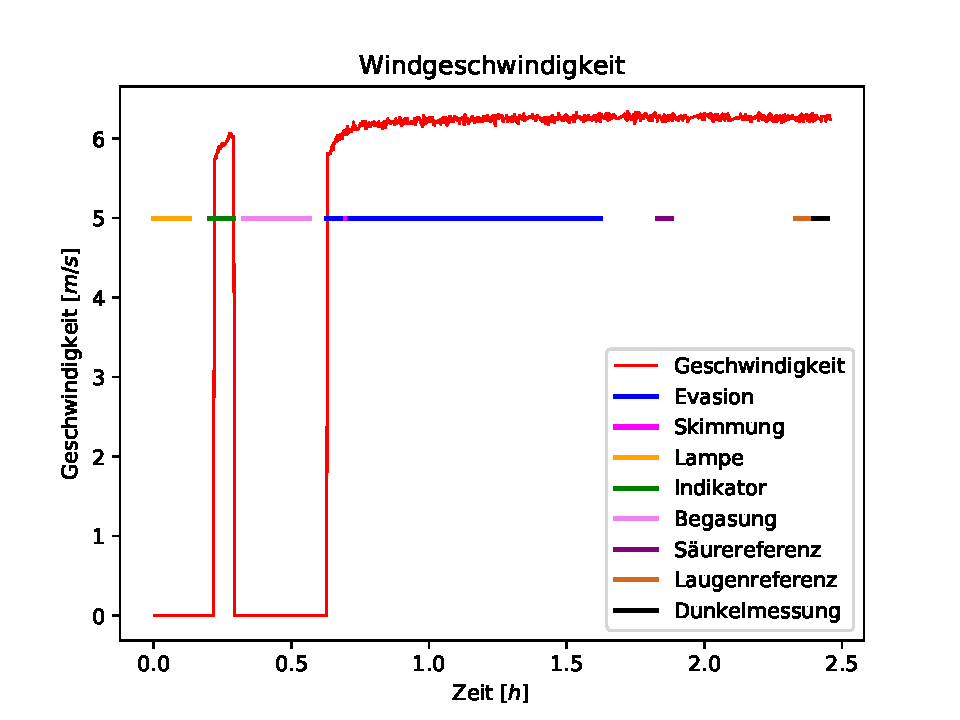
\includegraphics[width=82.5mm]{VE-Wasser/Windgeschwindigkeit}
		\caption{Windgeschwindigkeit}
	}
	\centering
	% hier schon der komplixiert Fall, dass 2 Bilder nebeneinander gesetzt werden
	\parbox{82.5mm}{
		\centering
		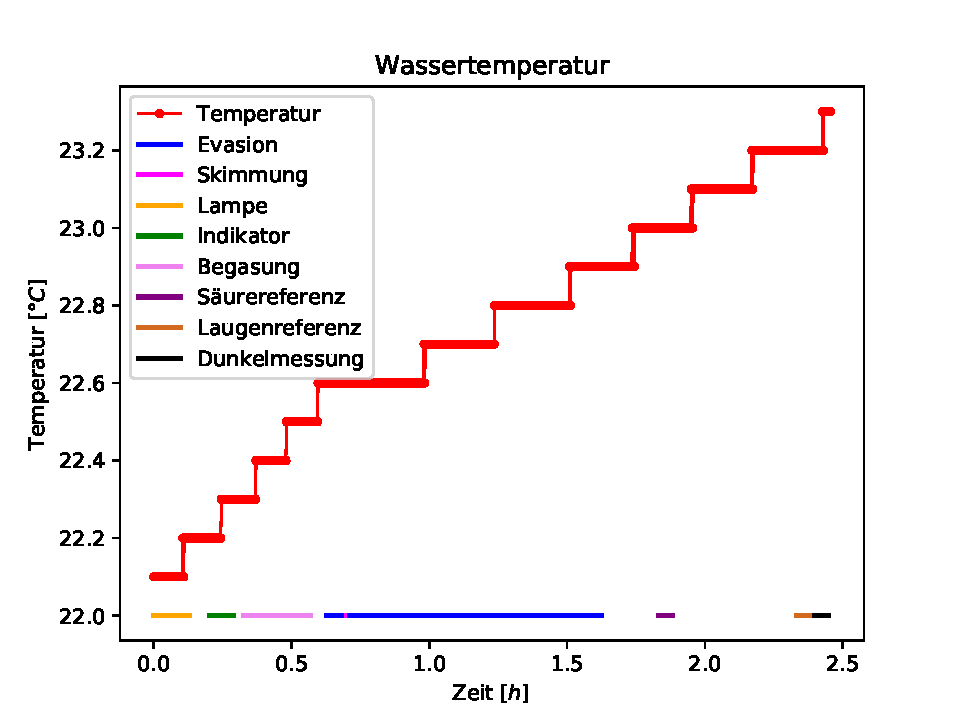
\includegraphics[width=82.5mm]{VE-Wasser/Wassertemperatur}
		\caption{Wasser- und Lufttemperatur}
	}
	\hfill% fuegt Platz ein, das rueckt die beiden Bilder an den Rand
	\parbox{82.5mm}{
		\centering
		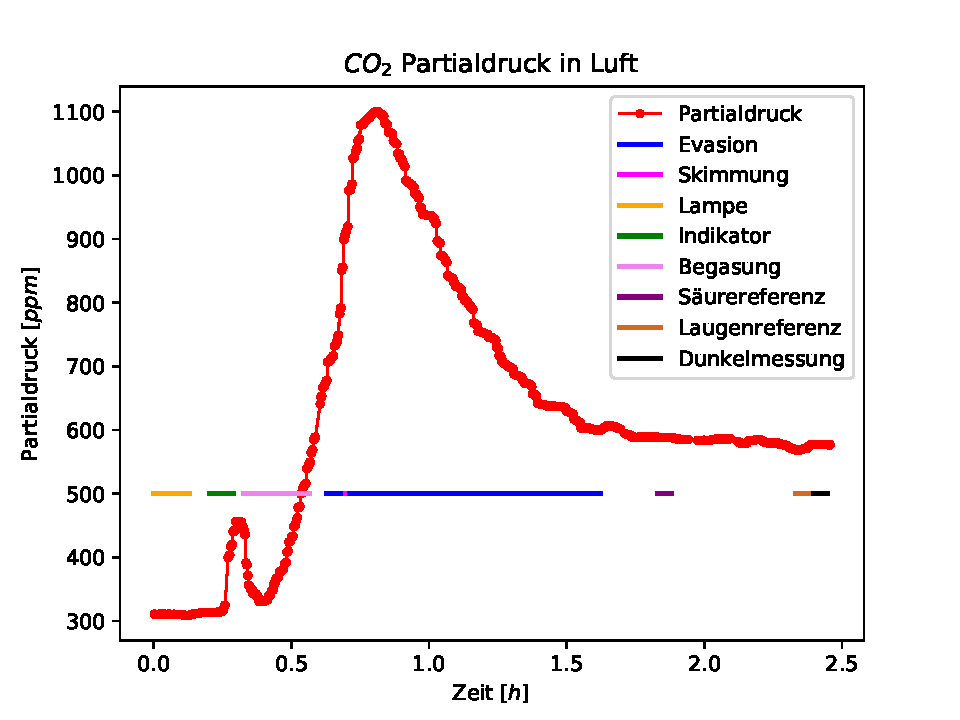
\includegraphics[width=82.5mm]{VE-Wasser/Partialdruck}
		\caption{Partialdruck von $CO_2$}
	}
	\centering
	% hier schon der komplixiert Fall, dass 2 Bilder nebeneinander gesetzt werden
	\parbox{82.5mm}{
		\centering
		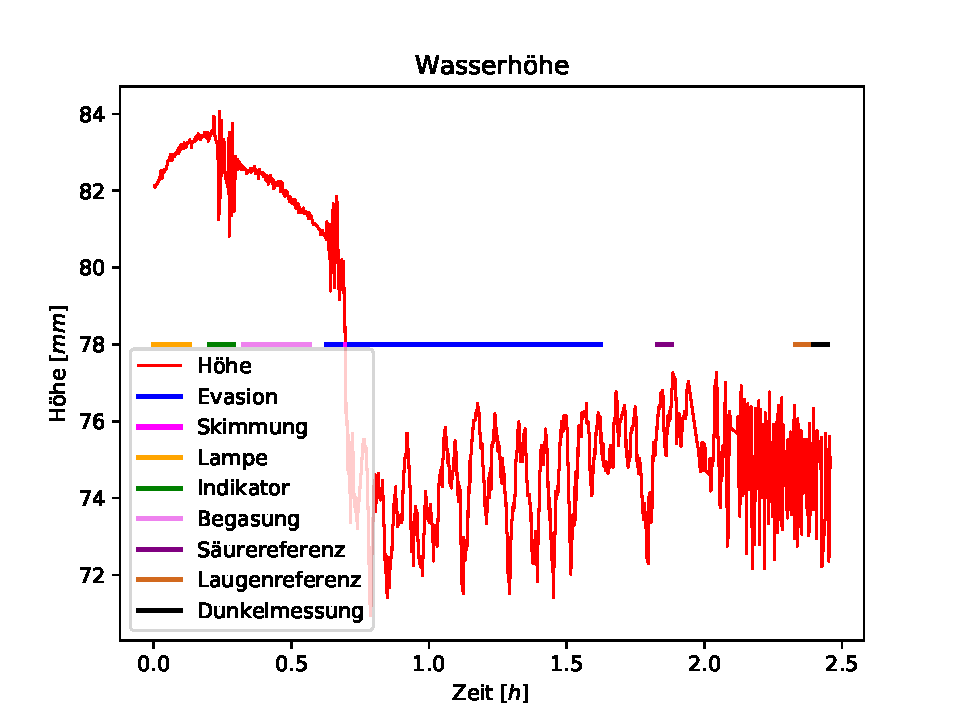
\includegraphics[width=82.5mm]{VE-Wasser/Wasserhoehe}
		\caption{Wasserh\"ohe }
	}
	\hfill% fuegt Platz ein, das rueckt die beiden Bilder an den Rand
	\parbox{82.5mm}{
		\centering
		%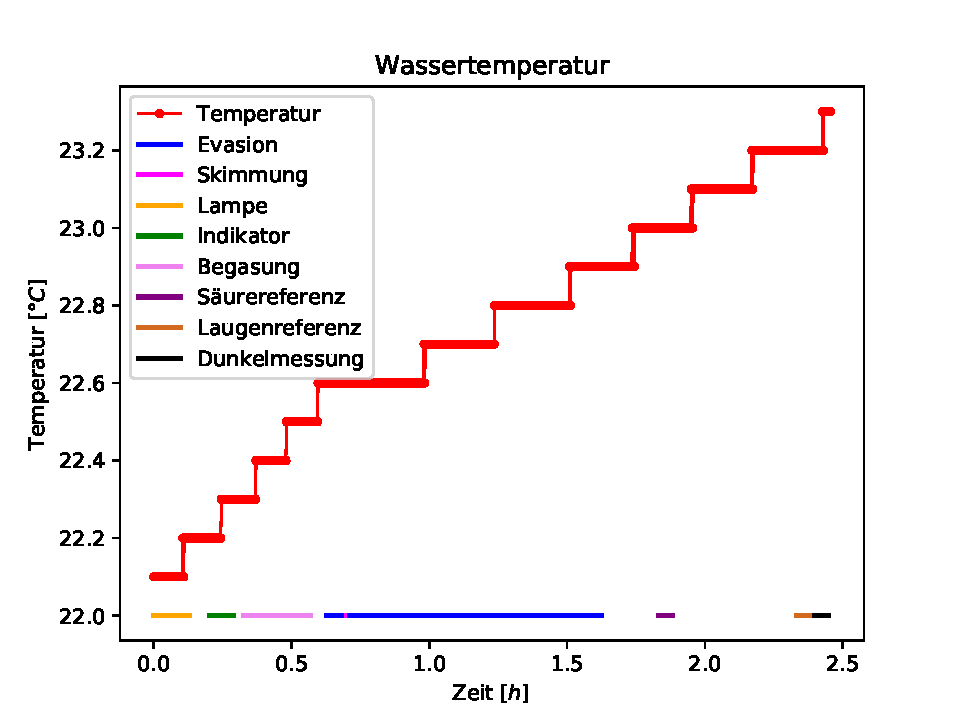
\includegraphics[width=82.5mm]{VE-Wasser/Wassertemperatur}
		%\caption{Wassertemperatur }
	}
\end{figure}

\paragraph{Diskussion der zeitlichen Verläufe\\}
%Intro
Die pysikalischen Parameter, Leitfähigkeit, Windgeschwindigkeit, $CO_2$-Partialdruck und die Wasserhöhe im Windkanal, sowie die Luft- und Wassertemperatur
wurden während der gesamten Zeit des Experiments aufgezeichnet, um Ergebnisse besser innerhalb ihrer physikalischen Rahmenbedingungen
erklären zu können. Zunächst erscheint es jedoch als notwendig, den Verlauf der Messdaten als solchen zu diskutieren.
%Windgeschwindigkeit
Der Verlauf der Windgeschwindigkeit (Abb. ???) beispielsweise zeigt deutlich auf, wann der Wind zu- und wann abgeschalten wurde. Während des
Umschaltvorgangs nimmt die Windgeschwindigkeit abrupt zu oder ab. Dies ist vor allem damit zu erklären, dass es im Luftraum sog.
Sekundärströmungen gibt. Das System ist vorwiegend turbulent, was zur Folge hat, dass nicht nur Gasbeimischungen schnell
verteilt werden, sondern auch der Impuls schnell transportiert wird. Die Windgeschwindigkeit nimmt daher überall im Kanal
schnell und mit der selben Rate zu bzw. ab. Dennoch ist auch zu beobachten, dass sich nach dem Anschaltvorgang die Windgeschwindigkeit
mit etwas Verzögerung auf einen finalen Wert einstellt. Das liegt daran, dass am Anfang der Impuls an das sich aufbauende Wellenfeld abgegeben wird
und auch der Wasserkörper durch die Windscherung langsam in Rotation versetzt wird. Irgendwann ist der Impulsübertrag vom Wind zum Wasser gleich
des Impulsverlustes des Wassers durch die Reibung an den Wännden des Windkanals, sowie durch interne Reibung und es stellt sich ein konstanter Wind ein.
%Luft- und Wassertemperatur
Auch eine Betrachtung der Luft- und Wassertemperatur (Abb. ???) ist sinnvoll. In beiden Fällen ist ein kontinuierlicher Anstieg aufgezeichnet.
Dies ist damit zu erklären, dass die Windmühle nicht thermisch isoliert ist und so Luft- und Wassertemperatur langfristig der in diesem Fall
höheren Umgebungstemperatur folgen. Das stufenartige Verhalten der Wassertemperatur ist auf eine grobe Auflösung des Messsensors zurückzuführen.
%Wasserhöhe
Nun zur gemessenen Wasserhöhe (Abb. ???). Diese schwankt sehr stark (Ausschläge von bis zu 15\% gemessen an der gesamten Wertespanne), was auch durchaus
so beabsichtigt wurde. Durch den eingestellten Wind werden innerhalb des Kanals Wellen erzeugt, die die Wassersäule teilweise massiv beeinflussen. Es wurden Wellen von etwa einem Zentimeter Höhe
beobachtet. Das entspricht bei einer Fülllhöhe von etwa sieben Zentimetern im Kanal bereits 15\%. Der überwiegende Abfall der Füllhöhe ist eigentlich
unerwünscht und durch eine undichte Stelle im Versuchsaufbau zu begründen. Es entwich über den ganzen Messungszeitraum Flüssigkeit aus dem Kanal, was
nicht wieder hinzugegeben wurde. Auch der Skimmvorgang zur Beseitigung der Oberflächenfilme (siehe ???) hat dafür gesorgt, das Wasser dem Kanalsystem entnommen,
jedoch nicht wieder hinzugegeben wurde. Eine solche Abnahme kann während der Zeit des Skimmens beobachtet werden.
%Partialdruck von CO_2
Der Partialdruck von $CO_2$ in der Luft ist in den Abb. ??? zu sehen. Er hängt direkt mit den am Experiment durchgeführten Eingriffen zusammen, die durch die horizontalen Balken
eingezeichnet sind. So ist etwa der größte Anstieg gefolgt von dem exponentiellen Abfall die Reaktion auf die Begasung des
Wassers mit sofortiger Evasion des $CO_2$ in die Luft. Der Abfall ist dann so zu erklären, dass durch die sinkende Gaskonzentration im Wasser auch
der abzugebende Teil an $CO_2$ an die Luft kleiner wird. Dadurch senkt sich der Partialdruck des Gases insgesamt.
Der kleinere Hochpunkt zu Beginn beider Messreihen ist mit \cite{jaehne} Abb. 8 zu verstehen. So ist die $CO_2$-Konzentration im VE-Wasser nie ganz
null, da durch den Ionentauscher nur geladene Teilchen herausgefiltert werden können. Gelöst liegen aber $CO_2, CO_3^{2-} $ und $HCO_3^-$ vor,
wovon $CO_2$ Moleküle nicht geladen sind und in Lösung bleiben. Dieser Anteil evasiert in die anfangs stehende Luft, der Partialdruck steigt.
%Leitfähigkeit
Die Leitfähigkeitsmessungen zeigen in Abb. ??? erst nach der Evasionsmessungen starke Veränderungen, was besonders durch die Zugabe von $HCl$ und $NaOH$
bewirkt wird. Dadurch befinden sich plötzlich viel mehr Ionen im Kanal, die durch die Messmethode registriert werden. Die Zugaben erfolgten jeweils
Schrittweise, was auch den gezackten Anstieg in den Plots erklärt. Der Abfall zwischen den beiden Peaks, der wieder in beiden Abbildungen vorkommt,
zeigt die Neutralisation von Salzsäure mit Natronlauge, also die Bindung der Ionen zu ungeladenen Molekülen, ehe weiter Lauge hinzugegeben wird. Auch
danach ist während der Messung eine konstante Menge Ionen vorhanden, was die Leitfähigkeit nicht ändert.



\subsubsection{Berechnung $CO_2$-Konzentration in Wasser nach Begasung}

Für die Konzentration des gelösten $CO_2$-Gases in Wasser wird berechnet, mit wieviel Mol an $CO_2$ das Wasser durch den Oxygenator begast wurde. Dazu werden folgende Formeln verwendet:

\begin{equation}
n = \dot V t \frac{\rho}{M}
\end{equation}

\begin{equation}
\Delta n = \sqrt{(t \frac{\rho}{M} \Delta \dot V)^{2}+(\dot V \frac{\rho}{M} \Delta t)^{2}}
\end{equation}

Mit Dichte: $\rho_{CO_2} = 1.98 \,\frac{kg}{m^3} $, molarer Masse: $M_{CO_2} = 44.0\,\frac{g}{mol} $, Zeit:  $t = (867 \pm 8) \, s$ und Massenfluss: $\dot V = (45.0 \pm 0.1)\,\frac{ml}{min}$ folgt daraus:

\begin{equation}
n_{w0} = (0.0293 \pm 0.0003) \,mol
\end{equation}

Ein Vergleich dieses Wertes mit dem durch die Löslichkeit von $CO_2$ in Wasser bestimmten Wert, um absch\"atzen zu können, ob das Wasser w\"ahrend der Begasung schon in S\"attigung war, liegt nahe. Das Volumen des Wassers in der Rinne betrug $V = 12.6 \,l $. Außerdem ist das Volumen des Leitungssystems von $V=1.1 \,l $ zu ber\"ucksichtigen. Die Berechnungsgrundlage hierfür bietet \cite{jaehne} Gleichung (44).
\begin{equation}
n = \alpha_{CO_2}(21 °C) \, V = 0.52 \, mol
\end{equation}

Wobei der Wert für die L\"oslichkeit aus \cite{jaehne} Abb. 4 verwendet wurde. Es kann also angenommen werden, dass sich die komplette begaste Stoffmenge an $CO_2$ in dem Wasser gelöst hat. Daraus ergibt sich für die anfängliche Konzentration:
\begin{equation}
c_{w0} = \frac{n}{V} = (2.11 \pm 0.02)\cdot 10^{-3} \frac{mol}{l}
\end{equation}

\subsubsection{Untersuchung Boxmodell-Bedingung}

Als theoretische Grundlage wird zur Untersuchung des Gasaustauschs vereinfachend das Boxmodell angenommen. Für dieses ist jedoch enscheidend, dass die Bedingung
$c_a \ll c_w/\alpha $ gilt. Ob überhaupt bzw. zu welchen Zeiten diese tatsächlich vorliegt, ist entscheidend um die Güte der darauf basierenden Aussagen einschätzen zu können.

\paragraph{Leitfähigkeitsmethode\\}

Zuerst folgt aus der Annahme $\Lambda ^2 \propto c_w $, dass $\Lambda ^2 = m \cdot c_w $. Danach wird also die Konstante $m$ gemäß
\begin{equation}
m = \frac{\Lambda^2(0)}{c_w(0)} = \frac{\Lambda^2(0)}{c_{w0}} = 37456 \frac{(\mu S)^2 l}{cm^2 mol} = 37.5 * 10^{-9} \frac{S^2 l}{cm^2 mol}
\end{equation}
bestimmt. Eine Berechung von $c_w$ für beliebige Zeiten ist damit möglich. Außerdem ist eine logarithmische Skalierung für die ins Verhältnis setzende Darstellung des Partialdrucks von $CO_2$ und der wasserseitigen $CO_2$-Konzentration von Vorteil, um die zwischen $c_a$ und $\frac{c_w}{\alpha}$ liegende Größenordnung abschätzen zu können.
Die Berücksichtigung der Löslichkeit in der Einheit $\frac{mol}{l}$ liefert den Partialdruck.

\begin{figure}[H]
	\centering
	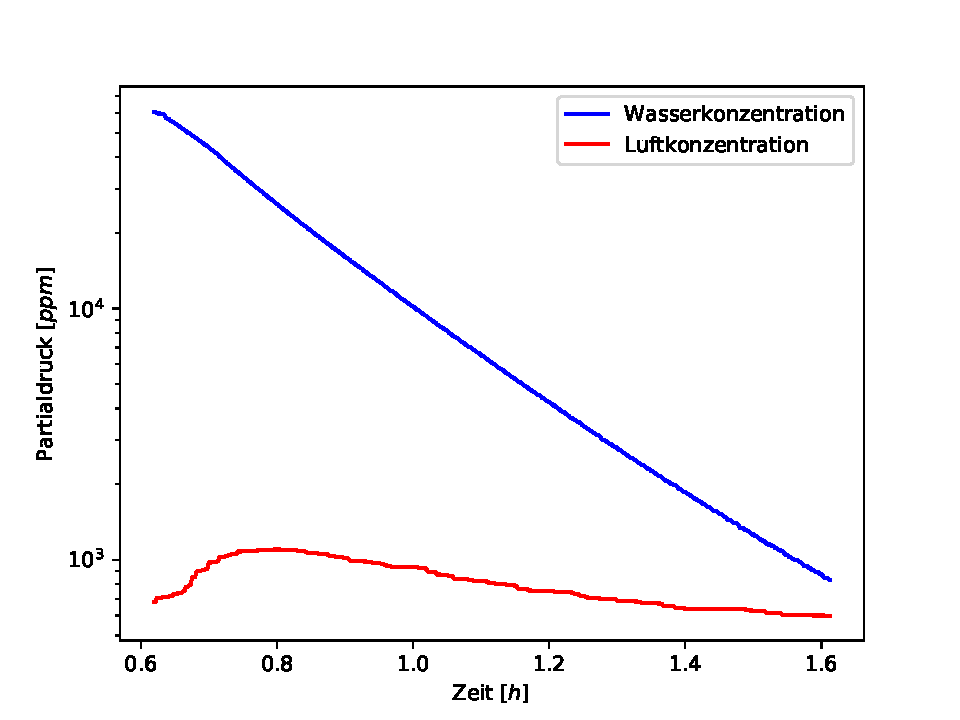
\includegraphics[width=120mm]{VE-Wasser/LeitfaehigkeitQuadrat.pdf}
	\caption{Konzentrationen während Evasion}
\end{figure}

In Abbildung 9 ist zu erkennen, dass bis zur Hälfte der Evasion die Bedingung $c_a \ll c_w/\alpha $ für das einfache Boxmodell deutlich erfüllt ist. Es liegt bis dahin
mindestens ein Verältnis von 1:10 zwischen den Konzentrationen vor. Zu Beginn der Evasion sogar eines von 1:100. \\\\
Eine Anmerkung ist an dieser Stelle noch zu machen. Die Messung des Partialdrucks von $CO_2$ weist mit ungefähr 170 ppm einen realtiv großen Offset auf.
Dessen Berücksichtigung hat jedoch für obige Beurteilung keine Relevanz, da die Verhältnisse nicht entscheidend beeinflusst werden.

\paragraph{Indikatormethode\\}

Auch für diese Methode wird eine Annahme über eine Proportionalität verwendet: $(\frac{[HI]}{[I^-]})^2 \propto c_w $, sodass $(\frac{[HI]}{[I^-]})^2 = m \cdot c_w $. Danach wird also die Konstante $m$ gemäß
\begin{equation}
m = \frac{(\frac{[HI]}{[I^-]})^2(0)}{c_w(0)} = \frac{(\frac{[HI]}{[I^-]})^2(0)}{c_{w0}}
\end{equation}
bestimmt. Hierbei soll (0) den Anfangszeitpunkt der Messung anzeigen. Mit Hilfe des Heurisko-Skripts können die Verhältnisse $\frac{[HI]}{[I^-]}$ für verschiedene Wellenlängenbereiche bestimmt werden.

\begin{figure}[H]
	\centering
	% hier schon der komplixiert Fall, dass 2 Bilder nebeneinander gesetzt werden
	\parbox{57.5mm}{
		\centering
		\begin{tabular}{c|c|c}
			$\lambda_1 [nm] - \lambda_2 [nm]$ & $\frac{[HI]}{[I^-]}(0)$ & $m [\frac{l}{mol}]$ \\ \hline
			284 - 836 & 2.51 & 2986 \\
			288 - 432 & 2.70 & 3455 \\
			524 - 880 & 2.49 & 2938 \\
			596 - 796 & 2.37 & 2662 \\
			304 - 376 & 2.75 & 3584
		\end{tabular}
		\caption{Übersicht der verschiedenen $\frac{[HI]}{[I^-]}$ und m für unterschiedliche Wellenlängenbereiche}
	}
	\hfill% fuegt Platz ein, das rueckt die beiden Bilder an den Rand
	\parbox{95mm}{
		\centering
		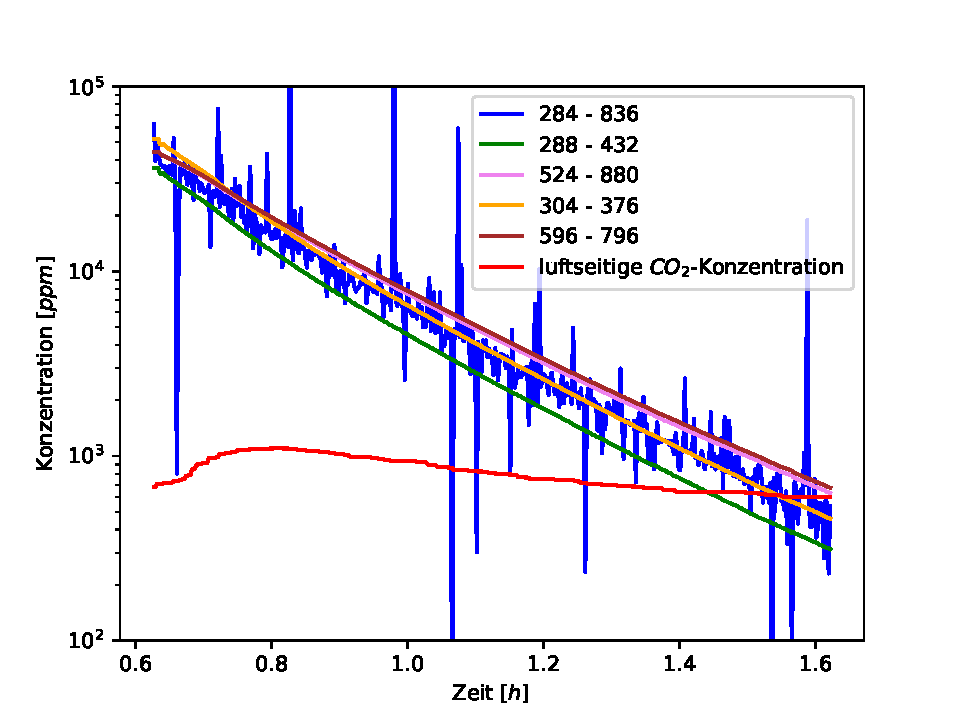
\includegraphics[width=95mm]{VE-Wasser/Indikator.pdf}
		\caption{Plot zur Abschätzung der Konzentrationsverhältnisse während Evasion für verschiedene $\frac{[HI]}{[I^-]}$ bzw. m}
	}
\end{figure}

Grundsätzlich liegt bei dieser Methode gegenüber der Leitfähigkeitsmethode ein ähnlicher Verlauf der Konzentrationsverhältnisse vor.
Unterschiede, welche aus den verschiedenen $\frac{[HI]}{[I^-]}$ bzw. verwendeten Wellenlängenbereichen resultieren, lassen sich jedoch erkennen.
Die Verwendung eines sehr großen Bereichs des Spektrums führt zu starken Verrauschungen, was vor allem daran liegt, dass auch die grünen Wellenlängen,
also der sensible Umschlagsbereich des Indikators verwendet werden. Warum dieser zu besonders großen Ausschlägen führt, lässt sich sehr gut mit Hilfe von
\cite{jaehne} Gleichung 37 verstehen. Ist die Lösung ungefähr so sauer wie alkalisch, wird der Zähler in der Gleichung sehr klein.
Veränderungen in den Intensitäten haben entsprechend relativ gesehen größere Auswirkungen. Außerdem sind die Intensitäten proportional zu
den Konzentrations- bzw. Ionenverhältnisse, was zu den in Abb. ??? erkennbaren Veränderungen führt. Abgesehen davon hat der verwendete
Wellenlängenbereich jedoch keinen großen Einfluss auf die Bewertung der Annahme. Das obige Ergebniss bleibt allgemein gültig. Mehr Details über die 
Spektren finden sich im anschließenden Kapitel.\\
Auch die in Abschnitt ??? getätigte Aussage über den nicht verwendeten Offset bleibt gültig. Dies erklärt ebenfalls, warum die Konzentration
im Wasser gegen Ende der Evasion scheinbar unter die in der Luft fällt.

\subsubsection{Spektren von VE-Wasser}

Mit Hilfe der Daten aus der Vorauswertung des Spektren-Bildes, welche mit dem Heurisko-Skript durchgeführt wurde, konnten die sauren und basischen
Referenzspektren, sowie das Lampen- und das Dunkelspektrum geplottet werden:

\begin{figure}[H]
	\centering
	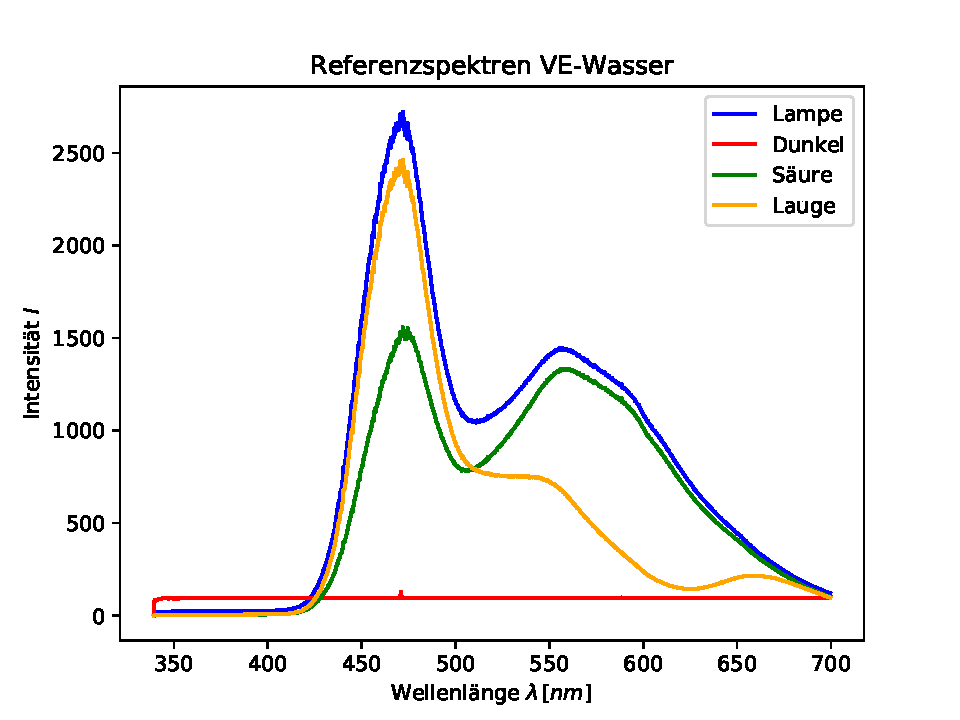
\includegraphics[width=120mm]{VE-Wasser/Referenzspektren}
	\caption{Plot der Spektren für VE-Wasser}
\end{figure}

\subsubsection{Bestimmung der Transfergeschwindigkeit in VE-Wasser mit der \\
Leitfähigkeitsmethode}

Ähnlich wie bei der Leitfähigkeitsmethode zur Abschätzung der Boxmodell-Bedingung wird auch dieses mal der Zusammenhang $\Lambda ^2 \propto c_w $ verwendet. Zusätzlich fließt in die Berechnung auch noch
\begin{equation}
c_w(t) = c_w(0) \cdot exp(-\frac{k}{h_{eff}}t)
\end{equation}
mit ein, was aus Gleichung (42) \cite{jaehne} entnommen wurde. Hierbei entspricht $k$ der gesuchten Transfergeschwindigkeit und $h_{eff}$ der effektiven Wasserhöhe, welche aus der gemessenen Wasserhöhe und dem Wasservolumen im Rohrsystem nach \cite{jaehne} (43) und (44) bestimmt wurde. Es ergibt sich also insgesamt folgender Zusammenhang:
\begin{equation}
k = -2 \frac{ln(\Lambda (t)/\Lambda (0))}{t} \cdot h_{eff}
\end{equation}
Das Verhältnis der Leitfähigkeiten wird logarithmisch geplottet, sodass aus der Steigung des Graphen die Transfergeschwindigkeit bestimmt werden kann. Bei den zwei Fits wurde einmal direkt über den kompletten Zeitbereich eine Exponentialfunktion angepasst und ein anderes Mal schrittweise für zwei Bereiche und dann die Transfergeschwindigkeit gemittelt.
Es wird $\Lambda (t)/\Lambda (0)$ aufgetragen, auch wenn es sich mit der Konzentration um einen quadratischen Zusammenhang handelt, da dieser bei logarithmischer
Betrachtung in einen Vorfaktor von 2 übergeht.

\begin{figure}[H]
	\centering
	% hier schon der komplixiert Fall, dass 2 Bilder nebeneinander gesetzt werden
	\parbox{82.5mm}{
		\centering
		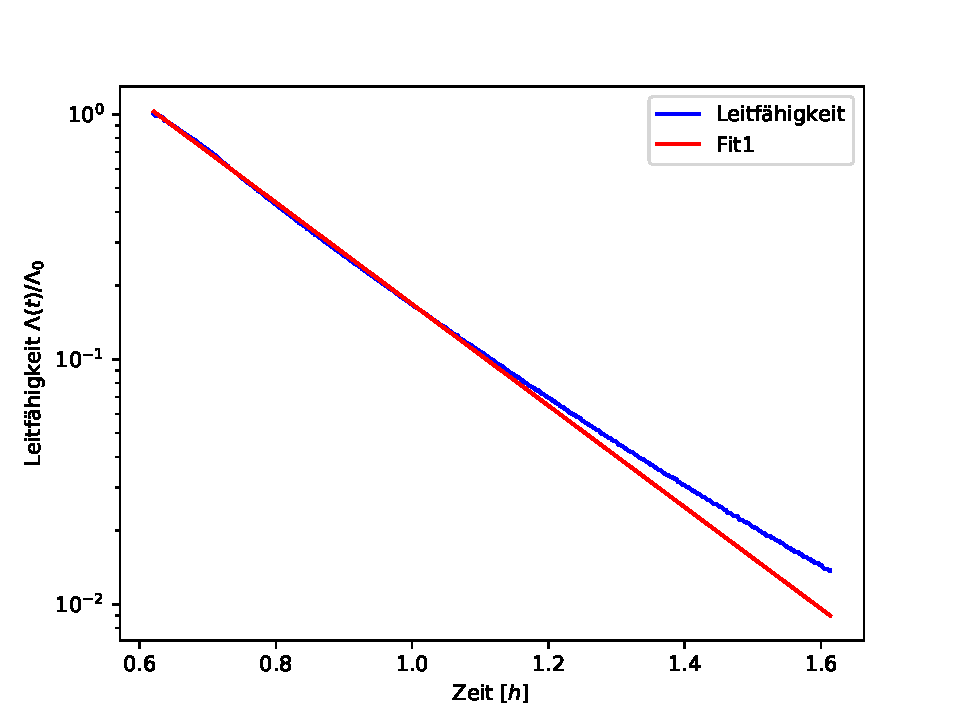
\includegraphics[width=82.5mm]{VE-Wasser/TransferGeschw}
		\caption{Durchgängiger Fit}
	}
	\hfill% fuegt Platz ein, das rueckt die beiden Bilder an den Rand
	\parbox{82.5mm}{
		\centering
		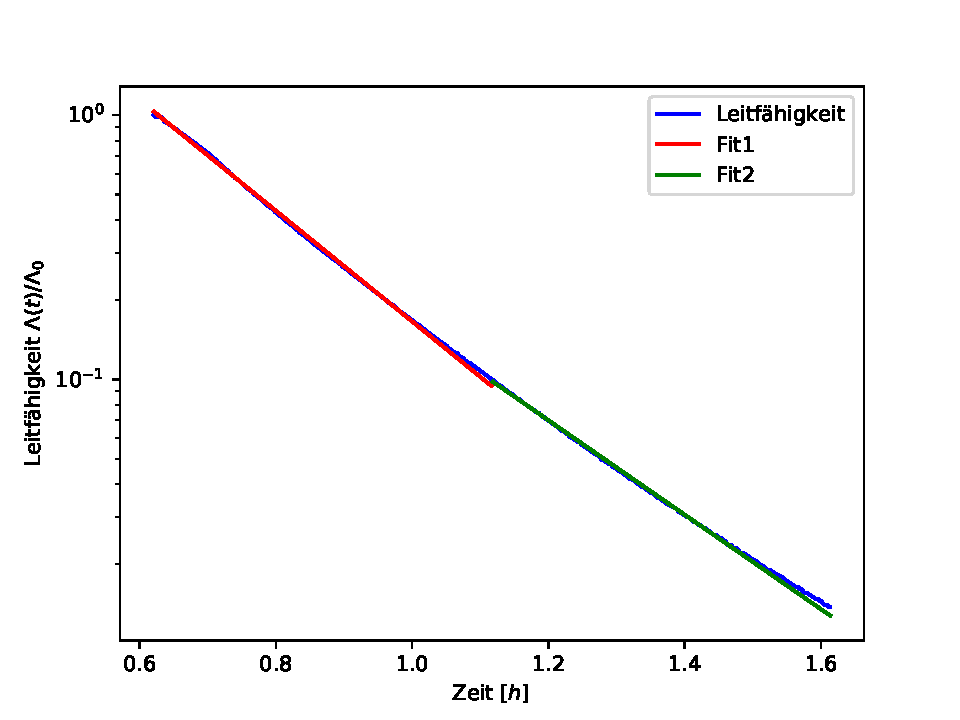
\includegraphics[width=82.5mm]{VE-Wasser/TransferGeschwKnick}
		\caption{Schrittweiser Fit (Halbierung der Fitbreite)}
	}
\end{figure}

 Es ergibt sich für den durchgängigen Fit:

\begin{equation}
	k = (38.9 \pm 0.8)\, \frac{cm}{h}
\end{equation}

Für den schrittweisen Fit folgt:

\begin{equation}
k_{ges} = (36.4 \pm 0.9)\, \frac{cm}{h}
\end{equation}

Hierfür wurden die stückweise berechneten Transfergeschwindigkeiten gemittelt:

\begin{equation}
k_1 = (39.2 \pm 0.8)\, \frac{cm}{h}
\end{equation}

\begin{equation}
	k_2 = (33.6 \pm 0.5)\, \frac{cm}{h}
\end{equation}

Die Unsicherheiten ergeben sich aus den Fitunsicherheiten. Außerdem muss bei dem zweiten Fit die Mittelung berücksichtigt werden.\\

Im Folgenden aufgeführte Messwerte dienen dazu obige Werte der Transfergeschwindigkeiten in einen physikalischen Kontext setzen zu können. Es wurden die Standardabweichungen bzw. Mittelwerte verwendet.

\paragraph{Durchgängiger Fit}
\begin{itemize}
	\item Wind: $v_w [\frac{m}{s}] = 6.22 \pm 0.06 $
	\item Wassersäule $h_w[mm] = 81.4 \pm 1.6 $
\end{itemize}
\paragraph{Schrittweiser Fit: Teil 1}
\begin{itemize}
	\item Wind: $v_w [\frac{m}{s}] = 6.19 \pm 0.06 $
	\item Wassersäule $h_w[mm] = 81.2 \pm 1.6 $
\end{itemize}
\paragraph{Schrittweiser Fit: Teil 2}
\begin{itemize}
	\item Wind: $v_w [\frac{m}{s}] = 6.26 \pm 0.03 $
	\item Wassersäule $h_w[mm] = 81.6 \pm 1.2 $
\end{itemize}

\subsubsection{Bestimmung Transfergeschwindigkeit in VE-Wasser - $\frac{[HI]}{[I^-]}$ Methode}
\begin{figure}[H]
	\centering
	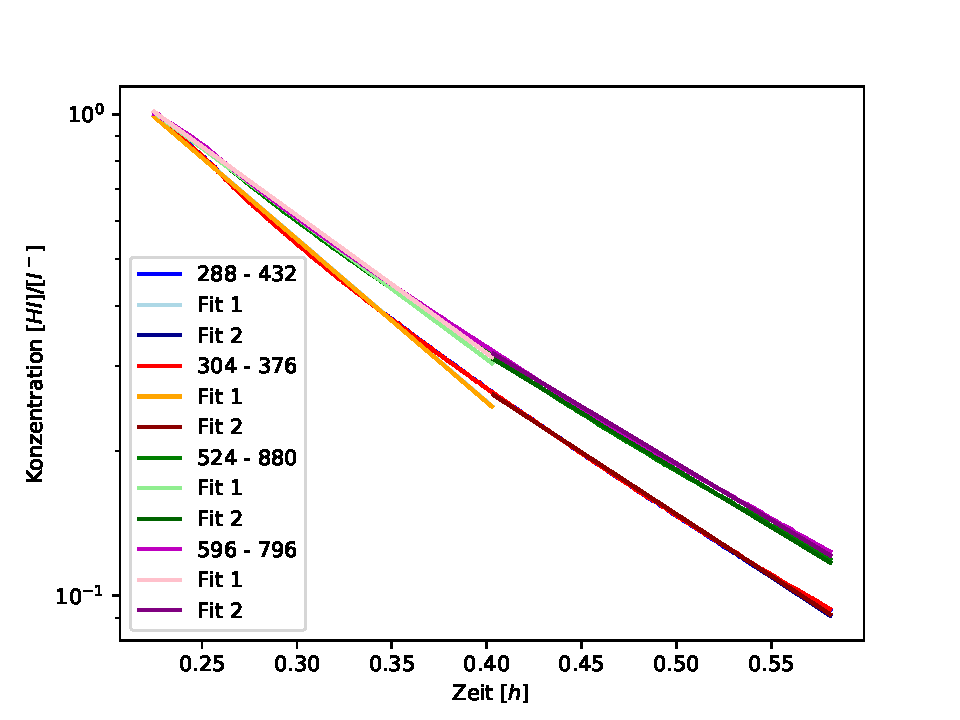
\includegraphics[width=120mm]{VE-Wasser/TransferhIKnick}
	\caption{Konzentrationen $\frac{[HI]}{[I^-]}$ über Zeit für verschiedene Wellenlängen mit Fits (Trennung bei $t \approx 0.4h$)}
\end{figure}

Aus der Steigung des Graphen wird nun wieder die Transfergeschwindigkeit nach der Indikatormethode bestimmt.
Daraus folgt für die Geschwindigkeit (siehe oben):
\begin{equation}
k = -2 \frac{ln(\frac{[HI]}{[I^-]}(t)/\frac{[HI]}{[I^-]}(0))}{t} \cdot h_{eff}
\end{equation}

Die einzelnen Transfergeschwindigkeiten aus den Fits der ersten Hälfte des Graphen, werden mit denen der zweiten Hälfte zu dem Wert $k_{ges} \, [\frac{cm}{h}]$ gemittelt.

\begin{figure}[H]
	\centering
	\begin{tabular}{c|c|c|c}
		Wellenlängenbereich $[nm]$ & $k_1 [\frac{cm}{h}]$ & $k_2 [\frac{cm}{h}]$ & $k_{ges} [\frac{cm}{h}] $ \\ \hline
		288 - 432 & $47.1 \pm 1.4$ & $35.2 \pm 0.5$ & $41.2 \pm 1.5$ \\
		304 - 376 & $47.2 \pm 1.4$ & $35.0 \pm 0.5$ & $41.1 \pm 1.5$ \\
		524 - 880 & $39.9 \pm 1.2$ & $32.5 \pm 0.5$ & $36.2 \pm 1.3$ \\
    	596 - 796 & $39.0 \pm 1.2$ & $32.2 \pm 0.5$ & $35.6 \pm 1.3$
	\end{tabular}
	\caption{Transfergeschwindigkeiten für unterschiedliche Wellenlängenbereiche}
\end{figure}

Auch aus dem zweiten Bereich wurden für die Evasion Tarnsfergeschwindigkeiten berechnet, auch wenn hier die Boxmodellbedingung nicht erfüllt ist. Dies dient
der späteren Diskussion. \\
Für die verschiedenen Bereiche, welche sich von denen bei der Leitfähigkeitsmethode unterscheiden, sind erneut die pysikalischen Messdaten gemittelt und
mit Standardabweichung aufgelistet.

\paragraph{Teil 1}
\begin{itemize}
	\item Wind: $v_w [\frac{m}{s}] = 6.1 \pm 0.5 $
	\item Wassersäule $h_w[mm] = 81.7 \pm 2.5 $
\end{itemize}
\paragraph{Teil 2}
\begin{itemize}
	\item Wind: $v_w [\frac{m}{s}] = 6.25 \pm 0.03 $
	\item Wassersäule $h_w[mm] = 81.5 \pm 1.2 $
\end{itemize}

\subsection{Meermodellwasser}
\subsubsection{Zeitliche Verl\"aufe der Messdaten}

\begin{figure}[H]
	\centering
	% hier schon der komplixiert Fall, dass 2 Bilder nebeneinander gesetzt werden
	\parbox{82.5mm}{
		\centering
		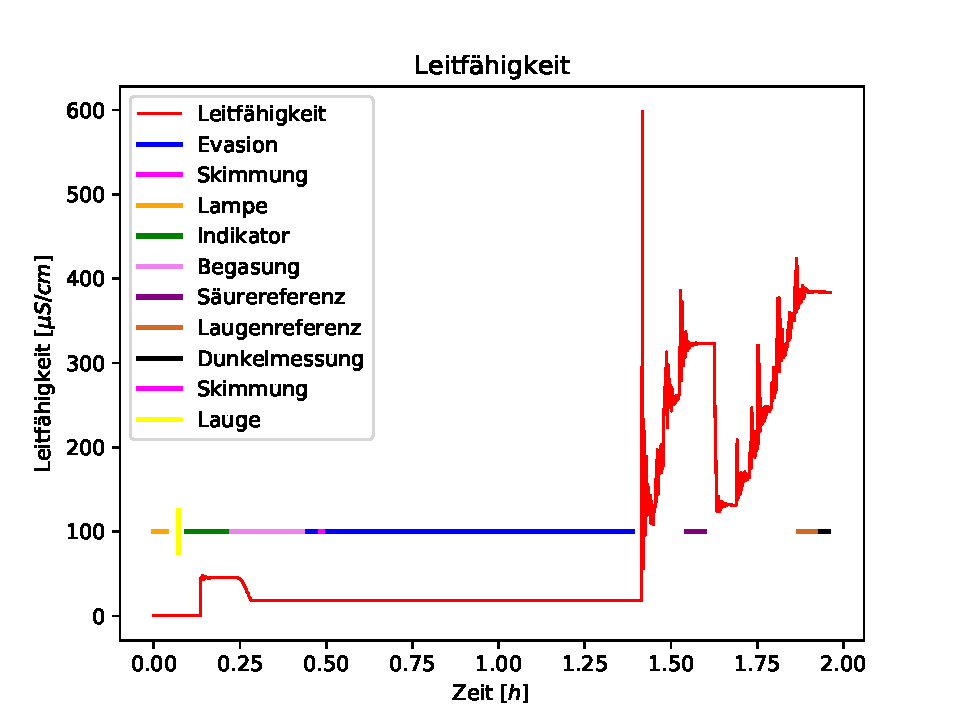
\includegraphics[width=82.5mm]{Meerwasser/Leitfaehigkeit}
		\caption{Leitf\"ahigkeit}
	}
	\hfill% fuegt Platz ein, das rueckt die beiden Bilder an den Rand
	\parbox{82.5mm}{
		\centering
		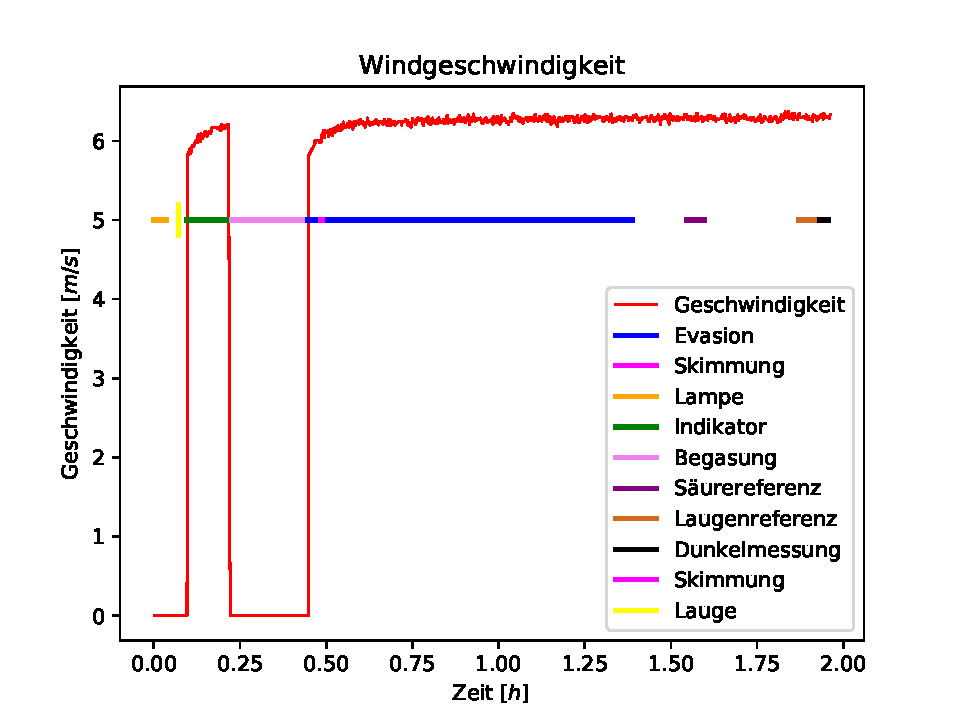
\includegraphics[width=82.5mm]{Meerwasser/Windgeschwindigkeit}
		\caption{Windgeschwindigkeit}
	}
	\centering
	% hier schon der komplixiert Fall, dass 2 Bilder nebeneinander gesetzt werden
	\parbox{82.5mm}{
		\centering
		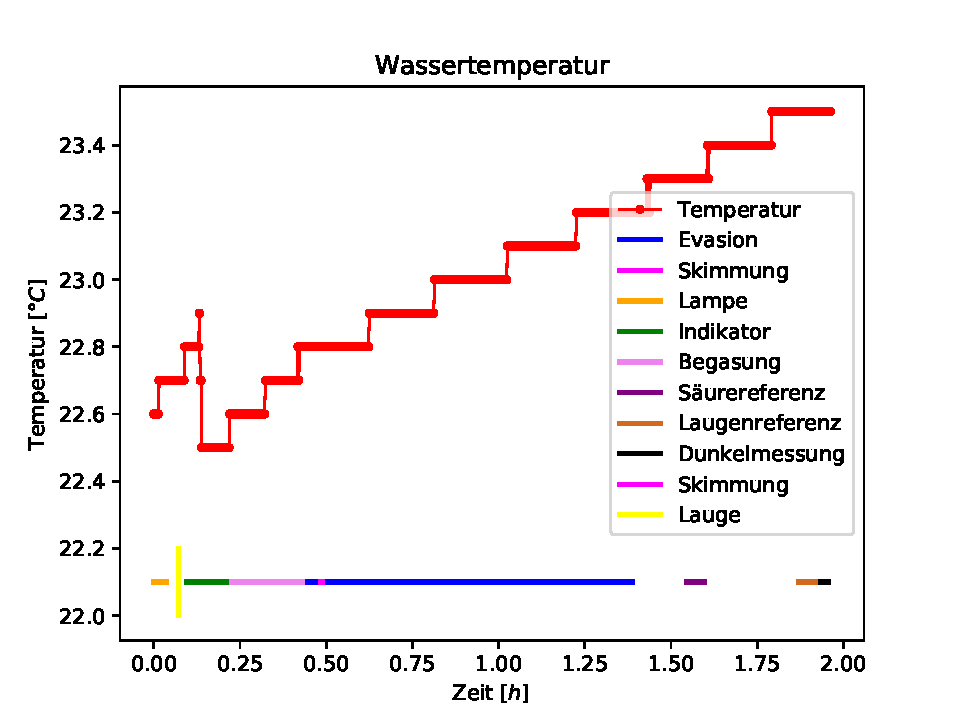
\includegraphics[width=82.5mm]{Meerwasser/Wassertemperatur}
		\caption{Wasser- und Lufttemperatur}
	}
	\hfill% fuegt Platz ein, das rueckt die beiden Bilder an den Rand
	\parbox{82.5mm}{
		\centering
		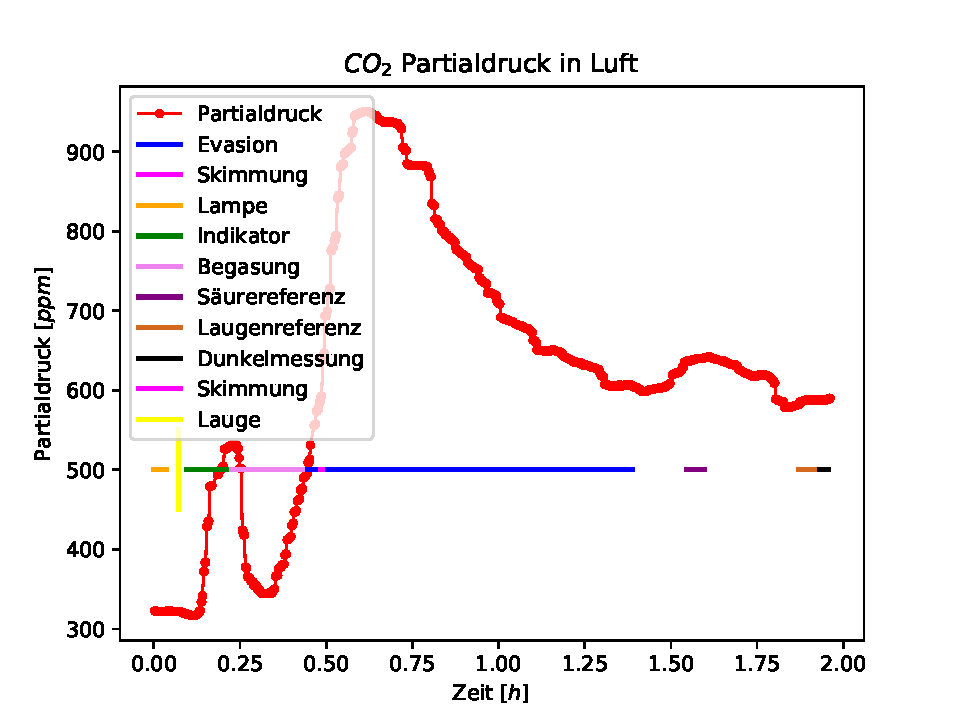
\includegraphics[width=82.5mm]{Meerwasser/Partialdruck}
		\caption{Partialdruck von $CO_2$}
	}
	\centering
	% hier schon der komplixiert Fall, dass 2 Bilder nebeneinander gesetzt werden
	\parbox{82.5mm}{
		\centering
		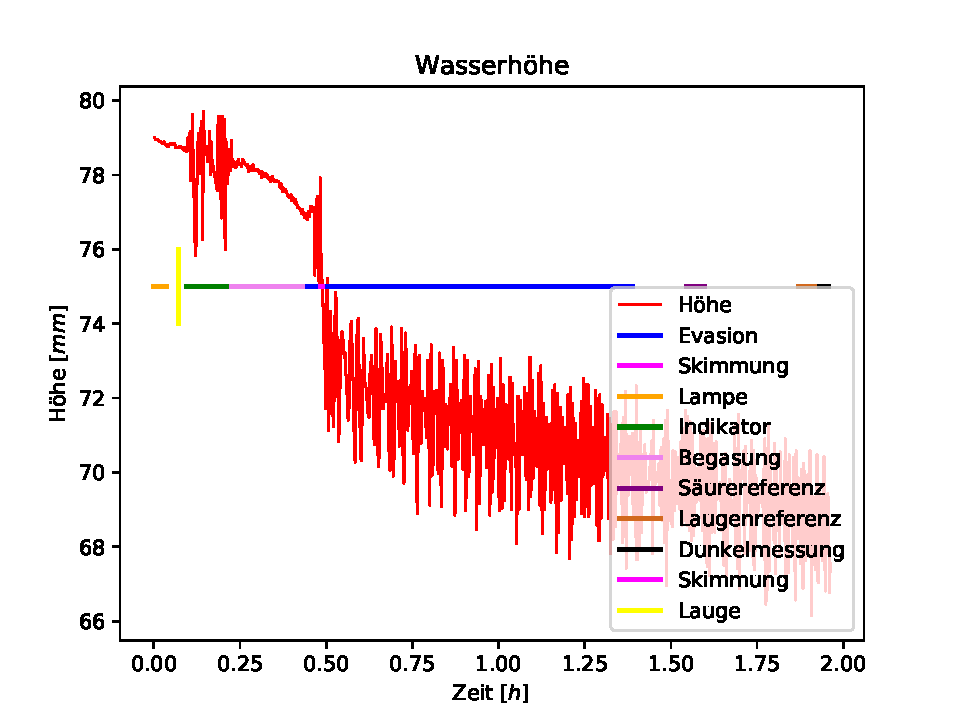
\includegraphics[width=82.5mm]{Meerwasser/Wasserhoehe}
		\caption{Wasserh\"ohe }
	}
	\hfill% fuegt Platz ein, das rueckt die beiden Bilder an den Rand
	\parbox{82.5mm}{
		\centering
		%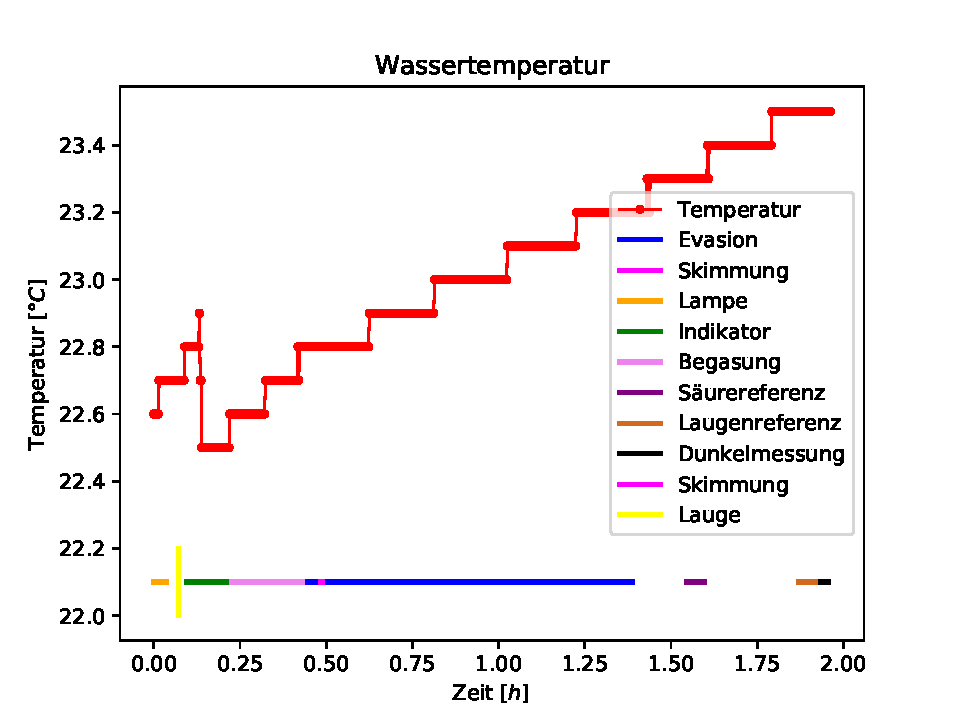
\includegraphics[width=82.5mm]{Meerwasser/Wassertemperatur}
		%\caption{Wassertemperatur }
	}
\end{figure}

%% Bilder: Sie sollten nicht versuchen, postscript 'from scratch' selbst zu
%% schreiben, sondern den Output von Analyseroutinen (PAW, ROOT, ...) oder
%% von Plot-Programmen (xfig, tgif) verwenden

\subsubsection{Berechnung $CO_2$-Konzentration in Wasser nach Begasung}

Analog zu der Berechnung der Anfangskonzentration bei VE-Wasser erfolgt die Berechung auch bei
Meermodellwasser. Folgende Werte liegen der Berechung in diesem Falle zugrunde: Dichte: $\rho_{CO_2} = 1.98 \frac{kg}{m^3} $, molarer Masse: $M_{CO_2} = 44.0\frac{g}{mol} $, Zeit:  $t = (737 \pm 8)s$ und Massenfluss: $\dot V = (45.0 \pm 0.1)\frac{ml}{min}$.\\

Es ergeben sich die beiden Zwischenergebnisse, $n_{w0} = (0.0249 \pm 0.0003) \,mol$ und $n = 0.52 \, mol$, woraus eine schlussendliche
Anfangskonzentration von $c_{w0} = (1.82 \pm 0.02)\cdot 10^{-3} \frac{mol}{l}$ folgt. Gegenüber der Anfangskonzentration bei VE-Wasser (siehe ???)
ergibt sich vor allem wegen der unterschiedlich langen Begasungszeit ein Unterschied.


\subsubsection{Untersuchung Boxmodell-Bedingung\\}

\paragraph{Indikatormethode\\}

Analog zu VE-Wasser wird auch hier die Proportionalität zwischen dem Verhältnis der Ionen und der Konzentration verwendet: $\frac{[HI]}{[I^-]} \propto c_w $, sodass $\frac{[HI]}{[I^-]} = m \cdot c_w $. Zu beachten ist, dass hier im Gegensatz zu VE-Wasser keine quadratische Proportionalität vorliegt, was auf den eingesetzen Indikator zurückzuführen ist.  \\

\begin{figure}[H]
	\centering
	% hier schon der komplixiert Fall, dass 2 Bilder nebeneinander gesetzt werden
	\parbox{57.5mm}{
		\centering
		\begin{tabular}{c|c|c}
			$\lambda_1 [nm] - \lambda_2 [nm]$ & $\frac{[HI]}{[I^-]}(0)$ & $m [\frac{l}{mol}]$ \\ \hline
			252 - 760 & 8.52 & 4681 \\
			264 - 368 & 10.37 & 5697 \\
			596 - 796 & 6.63 & 3643 \\
			496 - 764 & 7.25 & 3984 \\
			548 - 644 & 7.48 & 4110
		\end{tabular}
		\caption{Übersicht der verschiedenen $\frac{[HI]}{[I^-]}$ und m für unterschiedliche Wellenlängenbereiche}
	}
	\hfill% fuegt Platz ein, das rueckt die beiden Bilder an den Rand
	\parbox{95mm}{
		\centering
		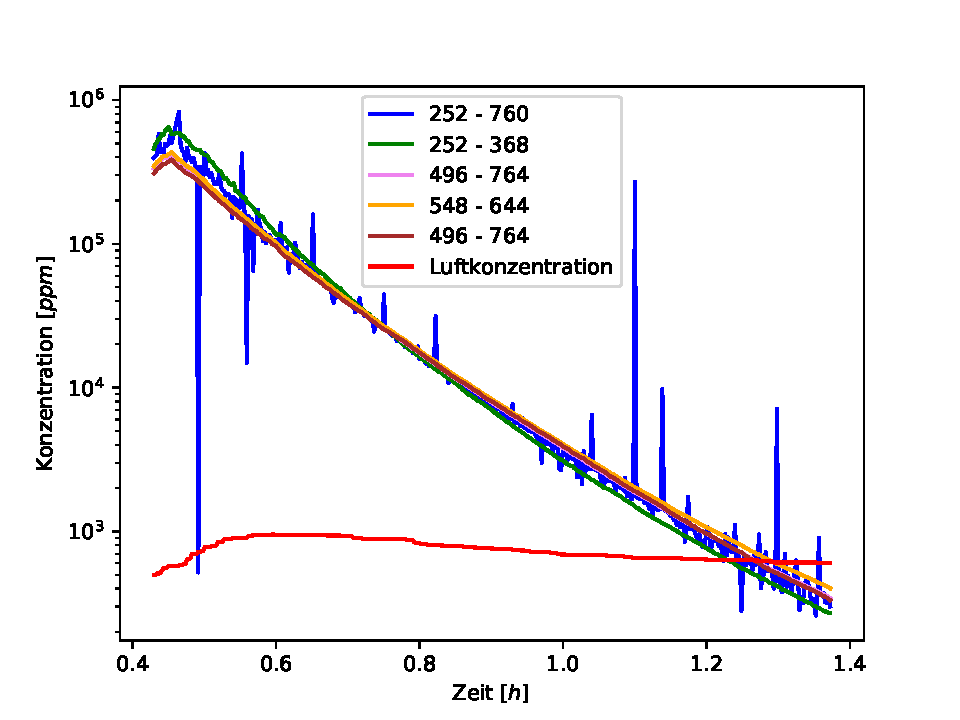
\includegraphics[width=95mm]{Meerwasser/Indikator.pdf}
		\caption{Abschätzung der Konzentrationsverhältnisse während Evasion für verschiedene $\frac{[HI]}{[I^-]}$ bzw. m}
	}
\end{figure}

Die Beobachtungen bezüglich der Bedingung $c_a \ll c_w/\alpha $ sind für das Meermodellwasser die gleichen wie für das VE-Wasser (siehe VE-Wasser/Untersuchung Boxmodell-Bedingung/Indikatormethode).

\subsubsection{Plot der Spektren}

\begin{figure}[H]
	\centering
	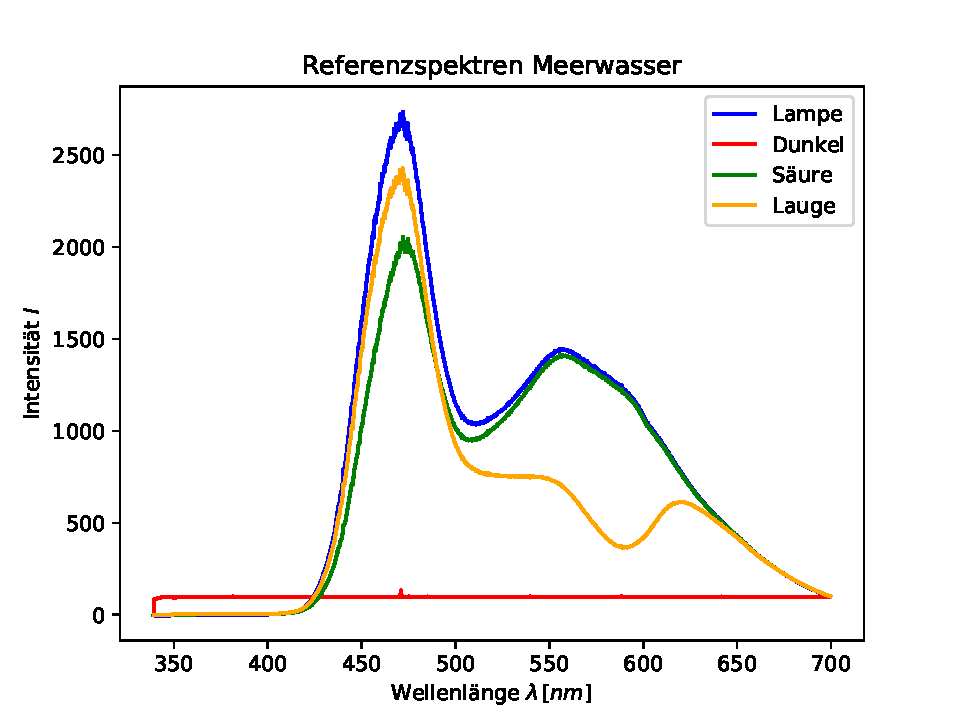
\includegraphics[width=120mm]{Meerwasser/Referenzspektren}
	\caption{Spektren für das Meermodellwasser}
\end{figure}

\subsubsection{Bestimmung Transfergeschwindigkeit - $\frac{[HI]}{[I^-]}$ Methode}
\begin{figure}[H]
	\centering
	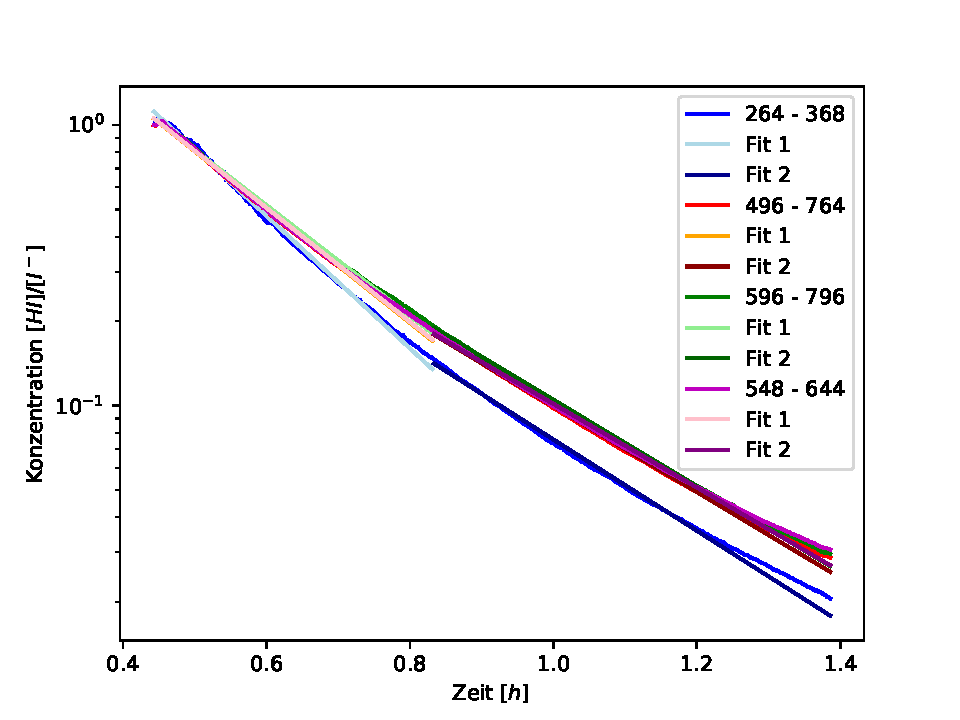
\includegraphics[width=120mm]{Meerwasser/TransferhIKnick}
	\caption{Konzentrationen $\frac{[HI]}{[I^-]}$ über Zeit für verschiedene Wellenlängen mit Fits (Trennung bei $t \approx 0.83h$)}
\end{figure}

Analog zum Vorgehen bei VE-Wasser wird auch dieses Mal die Steigung des Fits zur Bestimmung der Transfergeschwindigkeit
herangezogen, allerdings wie bereits bei der Untersuchung der Boxmodell-Bedingung unter Verwendung von $\frac{[HI]}{[I^-]} \propto c_w $.
Daraus folgt:
\begin{equation}
k = - \frac{ln(\frac{[HI]}{[I^-]}(t)/\frac{[HI]}{[I^-]}(0))}{t} \cdot h_{eff}
\end{equation}

Damit ergeben sich aufgeführte Werte:

\begin{figure}[H]
	\centering
	\begin{tabular}{c|c|c|c}
		Wellenlängenbereich $[nm]$ & $k_1 [\frac{cm}{h}]$ & $k_2 [\frac{cm}{h}]$ & $k_{ges} [\frac{cm}{h}] $ \\ \hline
		264 - 368 & $43.2 \pm 1.0$ & $29.1 \pm 0.5$ & $36.2 \pm 1.1$ \\
		496 - 764 & $37.3 \pm 0.8$ & $27.3 \pm 0.4$ & $32.3 \pm 0.9$ \\
		596 - 796 & $36.1 \pm 0.8$ & $27.4 \pm 0.4$ & $31.8 \pm 0.9$ \\
		548 - 644 & $37.1 \pm 0.8$ & $26.7 \pm 0.4$ & $31.9 \pm 0.9$
	\end{tabular}
	\caption{Transfergeschwindigkeiten für unterschiedliche Wellenlängenbereiche}
\end{figure}

\paragraph{Teil 1}
\begin{itemize}
	\item Wind: $v_w [\frac{m}{s}] = 6.1 \pm 0.8 $
	\item Wassersäule $h_w[mm] = 79.5 \pm 1.8 $
\end{itemize}
\paragraph{Teil 2}
\begin{itemize}
	\item Wind: $v_w [\frac{m}{s}] = 6.27 \pm 0.03 $
	\item Wassersäule $h_w[mm] = 77.6 \pm 1.2 $
\end{itemize}

\section{Diskussion}

% Intro
An dieser Stelle werden abschließend die Ergebnisse des Versuchs diskutiert.


Im nächsten Schritt wurde mit der Leitfähigkeitsmethode nur die Transfergeschwindigkeit für VE-Wasser bestimmt. Die Methode ist auf Meermodellwasser aufgrund der zustätzlich anwesenden Ionen nicht anzuwenden. Die berechneten Transfergeschwindigkeiten von $k = (38.9 \pm 0.8)\, \frac{cm}{h}$ bzw. $k_{ges} = (36.4 \pm 0.9)\, \frac{cm}{h}$ liegen im Bereich der später nach der Indikatormethode bestimmten Werte und auch im Bereich der Literaturwerte (\cite{jaehne} Abb. 6). Die angegebenen Ungenauigkeiten ergeben sich aus den Fits, sind jedoch, vergleicht man das schrittweise mit dem Komplett-Fit Vorgehen, deutlich höher anzusetzen. Das schrittweise Vorgehen erscheint hier deutlich genauer zu sein, was an der Güte der Fits ersichtlich wird. Hier wird der Verlauf deutlich besser beschrieben. Auch unterschiedliche Windgeschwindigkeiten oder Höhen der Wassersäulen könnten für Differenzen gesorgt haben. Vor allem die Windgeschwindigkeiten haben sich gemessen an ihren Ungenauigkeiten stark geändert. Seltsam erscheint jedoch die geringere Transfergeschwindigkeit im zweiten Teil der schrittweisen Methode, auch wenn dort die Windgeschwindigkeit höher war. Umgekehrtes ist nämlich zu erwarten. Vielleicht hat sich in dieser Zeit aber auch ein Oberflächenfilm gebildet, der von uns nicht bemerkt wurde und so für eine Dämpfung gesorgt hat. Mit Daten können wir dies jedoch nicht belegen, da der $mss$ der Wellen nicht gemessen werden konnte, anhand dessen Abnahme dies begründet hätte werden können.

Als nächster Punkt scheint wichtig, die gemessenen Spektren zu kommentieren. Zuerst soll dies für VE-Wasser geschehen. Der Dunkelstrom wurde bestimmt und bei den übrigen Spektren abgezogen. Als Referenzspektrum wurde das Spektrum der Lampe aufgenommen. Anhand dessen lassen sich Unterschiede der sauren und alkalischen Referenzspektren erkennen. Als Indikator wurde in diesem Fall Bromkresolgrün verwendet, welches im Umschlagpunkt grün, im Sauren gelb und im Alkalischen blau ist. All das lässt sich auch in den Referenzspektren erkennen. Der Schnittpunkt der beiden Referenzspektren liegt bei etwa 500 nm, was genau der Farbe des Indikators im Umschlagpunkt entspricht. Hier ist die Lösung sozusagen so sauer wie alkalisch, was sich in der gleich großen Intensität in den Spektren wiederspiegelt. Sowohl bei 470 nm (Blau) als auch ab 550 nm (Gelb) unterscheiden sich die beiden Referenzspektren stark. Hier dominiert jeweils das Spektrum, welches zu dem Milieu gehört, das durch den Indikator angezeigt wird. Entsprechend höher ist die Intensität.
Analoge Aussagen lassen sich für die Spektrenbilder des Meermodellwassers treffen. Hier wurde der Indikator Bromkresolpurpur verwendet, entsprechend ist der Umschlagpunkt eher im Blauen (480 nm) zu erkennen. Hier überwiegt auch das alkalische Referenzspektrum. Umgekehrtes gilt bei höheren Wellenlängen ab 550 nm, wenn auch der Indikator zunehmend rot wurde, was einem sauren Mileu entspricht.

% Bestimmung der Transfergeschwindigkeit
% Vergleich beider Messmethoden
Wie in der Auswertung zu sehen, kann die Transfergeschwindigkeit auf zwei unterschiedliche Arten gemessen werden. Dadurch wird ein Vergleich beider Methoden möglich, was jedoch nur für das VE-Wasser gilt. Eine der beiden benötigten Proportionalitäten gilt nur bei reinem Wasser und somit nicht für das Meermodellwasser.
Im Vergleich der Transfergeschwindigkeiten beider Methoden sieht man, dass der mittels Leitfähigkeit bestimmte Wert genau zwischen den Werten aus der Absorptionsmessung liegt. Hierbei zeigt sich, dass die Absorptionsmessung für verschiedene Wellenlängen recht unterschiedliche Werte liefert. Dabei spielen die später näher betrachteten Parameter, wie Wind und Wassersäule keine Rolle, da die Absorptionsspektren der einzelnen Wellenlängen exakt zu gleichen Zeiten aufgezeichnet wurden.
Durch die Annahme $c_w \propto \frac{[HI]}{[I^-]}$ ist hier nur der verwendete Indikator - Bromkresolgrün - entscheidend. Durch ihn wird das Licht abhängig von der $CO_2$ Konzentration beeinflusst.  Dazu können die Plots Abb. 15 \& 27 betrachtet werden. Auch hier zeigt sich nicht die gleiche Steigung der Geraden in der logarithmischen Darstellung, sondern die Konzentrationsabnahme ändert sich entsprechend der Wellenlängenbereiche. Hierbei ist zu beachten, dass dies vermutlich an den unterschiedlichen Referenzspektren liegt, die als Basis für die Berechung des Verhältnisses $\frac{[HI]}{[I^-]}$ verwendet wurden. Hauptsächlich für höherer Wellenlängen ergibt sich ein im Vergleich zum Lampenspektrum komplett unterschiedlicher Verlauf der Intensität für das alkalische Referenzspektrum. Dies könnte also die Ursache für die unterschiedlichen Transfergeschwindigkeiten sein, die aus $\frac{[HI]}{[I^-]}$ bestimmt werden. Warum das alkalische Referenzspektrum bei hohen Wellenlängen von der Form, wie auch von der Intensität sich so stark von dem Lampenspektrum unterscheidet hat vermutlich chemische Ursachen, auf die hier nicht genauer eingegangen werden kann. Angesprochene Unterschiede können bei Meermodellwasser bis zu beinahe 14\% erreichen, bei VE-Wasser sogar fast 16\%.

% Vergleich beider Wasserzusammensetzungen
Um die Wasserzusammensetzungen und auch die Einflüsse von Ionen im Wasser besser beurteilen zu können, bietet es sich an, die gemessenen Transfergeschwindigkeiten mittels der $\frac{[HI]}{[I^-]}$ Methode zu vergleichen. Dazu werden für die vier betrachteten Wellenlängenbereiche einzeln die Geschwindigkeiten gegenübergestellt.
Für niedrige Wellenlängenbereiche ($\lambda \approx 350 nm$) liegt die Transfergeschwindigkeit für VE-Wasser knapp 14\% höher als für das Meermodellwasser, für hohe Bereiche, also $\lambda \approx 700 nm$ ergibt sich die gleiche Abweichung der Modelle. Das heißt Meerwasser wird durch die zusätzlich vorhandenen Ionen im $CO_2$ Austausch eher gehemmt gegenüber einfachem $H_2O$.
Das macht in sofern Sinn, da $CO_2$ Moleküle in nicht ionisierter Form hauptsächlich in saurem Wasser vorliegen und nicht so sehr in Meerwasser, was in etwa einen pH-Wert von 8 hat.
Man kann diese Werte auch über die ablaufenden Reaktionen von $CO_2$ in Wasser anschauen:
Die Transfergeschwindigkeit ist höher, wenn das Verhältnis $\frac{[HI]}{[I^-]}$ schneller abnimmt. Daraus folgt, dass die Reaktion $HI \, + \, H_2O \rightleftharpoons \, I^- \, + \, H_3O^+$ schneller in die rechte Richtung ablaufen muss. Genau das passiert für neutrales Wasser schneller als für alkalisches Meerwasser.

% Einfluss der Parameter auf die Transfergeschwindigkeiten
Insgesamt kommt bei allen Berechnungen heraus, dass die Transfergeschwindigkeit zu Beginn der Evasionsmessung höher ist als gegen Ende. Dies sollte eigentlich nicht passieren, da die Transfergeschwindigkeit als Quotient aus Netto-Fluss und Konzentrationsdifferenz hier theoretisch konstant ist. Aus Gleichung 1 geht jedoch hervor, dass $k \propto h_{eff}$ gilt.
Wie in den Abbildungen 6 \& 21 zu sehen, nimmt die Wassersäule ab und damit sollte auch die Transfergeschwindigkeit geringer werden, was sie, laut Abb. 15 \& 27, tut.
Ein weiterer Einfluss existiert in dem Anstieg der Temperatur. Er ist über das gesamte Experiment etwa konstant und hat damit laut \cite{jaehne} Abb. 4 eine sinkende Löslichkeit zur Folge. Das wiederum hat einen größeren Einfluss auf die Transfergeschwindigkeit, je weniger die Invasion im Boxmodell mit $c_w \ll \alpha c_a $ vernachlässigt werden kann. Außerdem würde sich, wie ober bereits beschrieben dadurch der gesamte Formalismus ändern.
Auch die betrachtete Windgeschwindigkeit steigt über den Zeitraum der Evasionsmessung an, was ein Indiz für einen dicker werdenden Oberflächenfilm sein kann. Ein dickerer Oberflächenfilm hat dann eine stärker dämpfende Eigenschaft auf den Gasaustausch. Diese Annahme konnte jedoch nicht quantitativ bestätigt werden, da dazu eine funktionsfähige Wellenenigungsmessung nötig gewesen wäre. Mit bloßem Auge waren keine Änderungen des Wellenbildes erkennbar, doch sind bereits geringfügige Änderungen des Oberflächenfilms ausschlaggebend für die Transfergeschwindigkeit.

Letztlich ist die Ungenauigkeit der bestimmten Geschwindigkeiten sicherlich noch höher als in der Auswertung bestimmt. Es wurden hier nur die Standardabweichungen betrachtet, die bei den zugrunde liegenden großen Datensätzen kaum ausschlaggebend sind. Zwar war durch die lange Messzeit eine Mittelung über einen Zeitbereich möglich, wodurch der statistische Fehler gering wird, doch werden systematische Fehler gar nicht beachtet. Eine große Verfälschung der Messergebnisse wird erzielt, indem die Wechselwirkung des Wassers mit der Kanalwand gar nicht berücksichtigt wird. Bei dem großen Verhältnis von Oberfläche zu Wasservolumen wäre der Einfluss sicher nicht verschwindend.

Als letztes wird ein Vergleich mit den Literaturwerten (\cite{jaehne} Abb. 6) gemacht, wobei sich die Vergleichswerte aus dem Graphen ergeben mit einer Windgeschwindigkeit von $v_w = 6.0 \frac{m}{s}$
ergebenn. Zu sehen ist eine starke Abhängigkeit von der Windgeschwindigkeit. Dieser Graph deckt sich nun nicht perfekt mit den hier verwendeten Versuchsbedingungen, was wiederum den Wert des Vergleichs mindert, aber er bietet die beste vorliegende Vergleichbarkeit. Außerdem kann der Literaturwert nur mit einen großen Unsicherheit angegeben werden, da er nach Augenmaß aus der Abbildung ausgelesen werden muss.
\begin{equation}
	k = (34 \pm 2) \frac{cm}{h}
\end{equation}
Mit unseren Werten der Geschwindigkeiten für VE-Wasser ergeben sich Abweichungen von maximal $4 \sigma$. Für das Meermodellwasser dagegen sind die Abweichungen maximal im $2\sigma$-Bereich und somit nicht signifikant. Insgesamt ist auch hierzu zu sagen, dass die Ergebnisse wohl in einem guten Bereich liegen, beachtet man, dass die Bedingung für das Boxmodell ungefähr ab der Hälfte nicht mehr erfüllt ist, jedoch trotzdem der gleiche Formalismus verwendet wurde. Außerdem ist die Transfergeschwindigkeit stark davon abhängig, zu welchen Zeiten der Evasion sie bestimmt wird. Am Anfang ist sie deutlich höher als am Ende. In diesen Zeiten ist auch zu sehen, dass die Konzentration in der Luft schon beinahe so groß ist wie die im Wasser. Man könnte vermuten, dass es hier auch schon Rückkopplungen/Invasion gab. All das führt, wie oben bereits beschrieben zu deutlich höheren Unsicherheiten als die, welche sich aus den Fits ergeben. Dadurch verbessert sich die Güte der Ergebnisse nochmals.

\newpage
%% hier wird 'von Hand' eine neue Seite erzwungen

%% Literatur)

\begin{thebibliography}{00}   % {00}: max 2-stellige Referenznummer

\bibitem{jaehne} Bernd J\"ahne, F54 Versuchsanleitung (2017)

\end{thebibliography}

\end{document}
